\documentclass[a4paper]{article}

\usepackage{graphicx}
\usepackage{amsmath,amssymb}
\usepackage{minted}
\usepackage{multirow}
\usepackage{float}
\usepackage{algorithm}
\usepackage{algpseudocode}
\usepackage{todonotes}
\usepackage{forest}
\usepackage{xstring}
\usepackage{xcolor}
\usepackage[most]{tcolorbox}
\usepackage{xparse}
\usepackage{natbib}
\usepackage{adjustbox}

\usetikzlibrary{graphs,graphdrawing}
\usegdlibrary{layered}

% for external graphviz
\input{/home/donkarlo/Dropbox/repo/nd_language_ai_project/src/nd_language_ai/formal/computer/programming/tex/latex/code_clips/external_graphviz.tex}

% for tags
\input{/home/donkarlo/Dropbox/repo/nd_language_ai_project/src/nd_language_ai/formal/computer/programming/tex/latex/part/control_sequence/kind/semtag/semtag.tex}

% for links
\input{/home/donkarlo/Dropbox/repo/nd_language_ai_project/src/nd_language_ai/formal/computer/programming/tex/latex/code_clips/seehere.tex}

% for nested lists and sections
\input{/home/donkarlo/Dropbox/repo/nd_language_ai_project/src/nd_language_ai/formal/computer/programming/tex/latex/code_clips/deep_structure.tex}

\title{}
\date{}
\author{Mohammad Rahmani}

\begin{document}
   \maketitle

   \seeherefooter{https://deutsch.lingolia.com/en/listening/b1/articles/bahnhof-train-station}

   Transcript

   Auf dem Bahnhof
   Das ist ja gerade noch einmal gut gegangen! Wir sitzen im Zug und können uns auf den Urlaub freuen. Aber beinahe hätten wir unseren Zug verpasst. Was ist passiert?

   Wir kamen pünktlich am Bahnhof an, und erkundigten uns zuerst an der Anzeigetafel, von welchem Gleis unser Zug abfährt. Dann gingen wir zum Fahrkartenautomaten und kauften unsere Fahrkarten und Platzkarten.

   Wir hatten noch ein wenig Zeit, also schlenderten wir gemütlich über den Bahnhof. Als wir schließlich auf unserem Bahnsteig ankamen, stand dort ein Güterzug. Das konnte doch nicht sein! Hier sollte doch unser Zug stehen!

   Dann erfuhren wir, dass unser Zug heute von Gleis 8 abfährt. Oje! Es war schon spät, wir hatten nur noch zwei Minuten bis zur Abfahrt. So schnell wir konnten, rannten wir quer über den Bahnhof, denn über die Schienen darf man nicht gehen. Als wir auf Gleis 8 ankamen, schaute der Lokführer aus der Lokomotive heraus und wollte gerade abfahren. Der Schaffner war aber so freundlich und wartete auf uns. Wir waren die letzten Passagiere.

   Schnell stiegen wir in den ersten Wagen ein. Aber für diesen Wagen hatten wir keine Platzkarten. Um unsere Sitzplätzen zu erreichen, mussten wir mit unserem Gepäck durch den ganzen Zug und sogar durch den Speisewagen.

   Aber wenigstens hatten wir den Zug nicht verpasst.
   \begin{figure}[H]
      \centering
      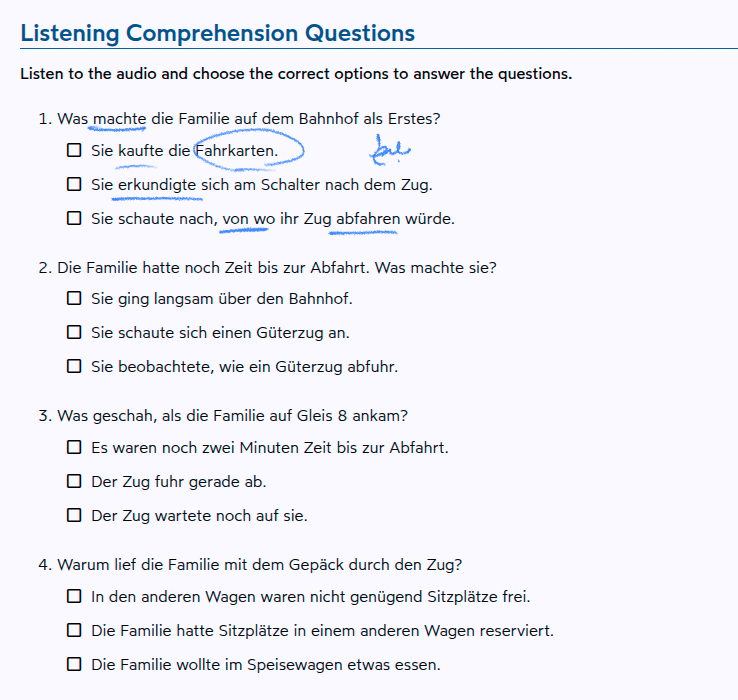
\includegraphics[width=0.9\textwidth]{img_0.png}
   \end{figure}
   \bibliographystyle{plainnat}
   \bibliography{/home/donkarlo/Dropbox/repo/nd_shared_research/bibliography/bibliography.bib}
\end{document}
